\documentclass[10pt]{article}
\usepackage[dvipsnames]{xcolor}
\usepackage{listings}
\usepackage{tikz}
\usepackage{url}
\usepackage{multicol}
\usepackage{xspace}
\usepackage{pstricks}
\usepackage{textcomp}
\usepackage[default]{droidserif}
\usepackage[T1]{fontenc}

%\usepackage{algorithm2e}
\usetikzlibrary{arrows,automata,shapes}
\tikzstyle{block} = [rectangle, draw, fill=blue!20, 
    text width=2.5em, text centered, rounded corners, minimum height=2em]
\tikzstyle{bw} = [rectangle, draw, fill=blue!20, 
    text width=4em, text centered, rounded corners, minimum height=2em]

\newcommand{\handout}[5]{
  \noindent
  \begin{center}
  \framebox{
    \vbox{
      \hbox to 5.78in { {\bf ECE155: Engineering Design with Embedded Systems } \hfill #2 }
      \vspace{4mm}
      \hbox to 5.78in { {\Large \hfill #5  \hfill} }
      \vspace{2mm}
      \hbox to 5.78in { {\em #3 \hfill #4} }
    }
  }
  \end{center}
  \vspace*{4mm}
}

\newcommand{\lecture}[4]{\handout{#1}{#2}{#3}{#4}{Lab #1}}
\topmargin 0pt
\advance \topmargin by -\headheight
\advance \topmargin by -\headsep
\textheight 8.9in
\oddsidemargin 0pt
\evensidemargin \oddsidemargin
\marginparwidth 0.5in
\textwidth 6.5in

\newcommand{\todo}[1]{{\red\textbf{TODO: }#1}\xspace}

\parindent 0in
\parskip 1.5ex
%\renewcommand{\baselinestretch}{1.25}

\begin{document}

\lecture{3 (Dead Reckoning)}{Spring 2014}{Prepared by Kirill Morozov}{version 1.1}

{ \bf Deadline:} You must submit the lab to the SVN repository by the submission deadline (see the syllabus) and be
prepared to demonstrate Lab 3 to a TA at the start of your first assigned
Lab 4 session.  The best way to demo is during a lab session, but any
earlier time where you can convince a TA to watch is OK too.

\begin{figure}[h]
\begin{center}
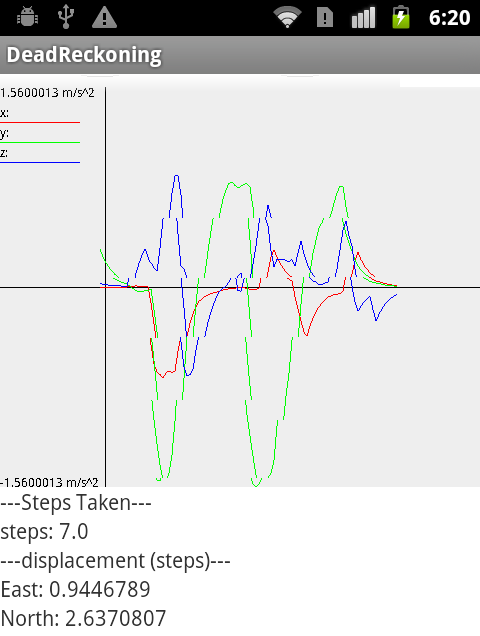
\includegraphics[width=0.25\textwidth]{device-screenshot-lab-3.png}
\end{center}
\caption{\label{fig:lab-3-screen}A complete lab 3 implementation.}
\end{figure}

\section{Objectives}
The goal of this lab is to integrate readings from multiple sensors to make more complex conclusions. In particular, you will combine your solution from lab 2 with readings from your Android phone's compass to track which direction the user is walking in. The solution for Lab 3 will tell the user the distance travelled from the starting point.

During this lab, you will:
\begin{enumerate}
\item Filter raw sensor data to account for noise and bias.
\item Study raw rotation readings to identify patterns.
\item Read information about the phone's heading.
\item Combine sensor readings to track a user's displacement.
\item Load the map (but you don't have to make use of it yet).
\end{enumerate}

\newpage
\section{Background}

This lab builds on what you learned in Labs 1 and 2. Most students will probably start with their Lab 2 code as a template. The following information may be helpful in completing this lab:

\paragraph{Compass error sources.}
For this lab, you will be using the {\tt SensorManager.getOrientation()} method to figure out how the user is oriented relative to the physical world. There are a number of pitfalls to avoid here. First, calculating the orientation of the phone relies on the phone's magnetic field sensor to find magnetic north. So, when you're close to magnetic objects (your computer's speakers, the big green power boxes in the Davis Centre or even the re-bar in the concrete walls), your orientation sensor's readings will be off. We will take this into account when running the lab demos, but you should keep this in mind when testing your application.

\paragraph{Compass calibration.}
The magnetic field sensors (and hence the compass readings) seem to get stuck sometimes such that they consistently return bogus values. Rotating the phone 1--2 times along each of its axes often fixes this. Alternately, there's also mention of drawing some sort of figure-8 in the air with the phone. People on the Internet call this ``calibration''.

\paragraph{Compass noise.}
You will notice that, like the accelerometer, the orientation sensor also has noise. However, you can't directly filter or average the results of your {\tt getOrientation()} calls. This sensor differs from the accelerometer from Lab 2 because the values for the azimuth (the rotation around the X axis) are reported modulo 2$\pi$. For example, if the phone reports that its azimuth is 2$\pi$ at time $t$ and 0 at time $t+1$, then averaging those values together will give you the completely wrong answer.

A particular danger of taking your bearing at the same point of every step is systemic bias. If you choose to make a widget to draw a compass on the screen (not required), you may notice that it consistently jumps wildly at a particular point of each step. Hence, taking the compass bearing at the same point in each step carries the danger of sending you way off course.

One way to solve this problem is to find a way to average data independent of the data's actual value---you'll want to use only its relative value. For example, at time $t=n$ you can take the value of your variable, and call that the base-line. Then, for some number of samples, you take the average of the (signed) distance between the samples and the base-line.

Another potential solution is to just take periodic sensor readings
and trust (or ensure, e.g. via randomness) that these aren't in
resonance with the tester's step frequency.

\paragraph{Determining direction.}
We can think of two ways to determine which direction the user is walking in. You can either assume that the user is always moving in the direction that the phone is pointed at (its heading), or you can look at the direction the phone is accelerating. Using the output acceleration is tricky because of the rotation problem, as discussed below. Just using the phone's heading is sufficient for this lab and for lab 4. 

\section{The Rotation Problem}
In lab 2, you probably noticed that if you rotate the phone on its axis, you get spikes of acceleration on one axis of the phone, but no corresponding counter-spike when the phone stops. We understand that this is a limitation of the accelerometer hardware, which is not set up to detect angular acceleration. In principle, one should be able to detect rotation using the rotation sensor, and account for rotation-based acceleration that way. However, our experience is that the rotation sensor data on the Nexus One phones is too noisy. We believe that this is because the Nexus One does not have an actual gyroscope---its rotation sensor is implemented in software by integrating data from the compass and accelerometer. 

However, it should be possible to solve the rotation problem if you have a phone with a gyroscope. If you can find a way to mitigate errors in the rotation data, either by using a gyroscope, or by doing something clever with the accelerometer data, you will get a bonus on this lab. You will need to output your filtered linear acceleration into a graph view during your demo to show that you are correctly filtering your data.

\section{The Map of the Real World}
For this lab, we will provide you with the {\tt MapView} Java class. The {\tt MapView} enables the user to select a starting point and a destination on an interactive map. We will also provide you with map files of the testing area (our lab room, E2-2364) ready for use by the {\tt MapView}. 

You can find the complete {\tt mapper} package in the SVN repository under \url{materials/mapper}. Copy this package into your project. The {\tt MapView} provides enough functionality to complete lab 3 and 4. However, if you would like to modify the mapper to make it prettier or to add additional functionality, go ahead! (For instance, you could implement multitouch functionality to zoom your map.)

\paragraph{Setting up the MapView.} The {\tt MapView} is an Android {\tt View}, like the {\tt LineGraphView} from Lab~1. Thus, you can use the techniques from Lab 1 to add the {\tt MapView} to your applications. 

Here's what the {\tt MapView} needs.
The {\tt MapView}'s constructor takes five parameters. The first, the application context, is common to all {\tt View}s. The second and third parameters are the width and height of the mapper in pixels. The fourth and fifth parameters are the X and Y scale that should be used to display the map. The scale is represented as pixels displayed per meter represented. As an example:

\begin{lstlisting}[basicstyle=\ttfamily\small]
    MapView mv = new MapView(getApplicationContext(), 400, 400, 60, 60)
\end{lstlisting}
\vspace*{-1em}
You will need to tune the parameters so that the map fits on your phone screen.

The {\tt MapView} comes with a context menu; add the following lines to your application to use it: 

\begin{lstlisting}[basicstyle=\ttfamily\small]
    // In your Activity's onCreate() method:
    registerForContextMenu(mapView);

    // In your Activity:
    @Override
    public void onCreateContextMenu(ContextMenu menu, View v, ContextMenuInfo menuInfo) {
    	super.onCreateContextMenu(menu, v, menuInfo);
    	mv.onCreateContextMenu(menu, v, menuInfo);
    }

    @Override
    public boolean onContextItemSelected(MenuItem item) {
    	return super.onContextItemSelected(item) || mapView.onContextItemSelected(item);
    }
\end{lstlisting}
\vspace*{-2em}

\paragraph{Loading a map.} The {\tt MapView} accepts SVG (Scalable Vector Graphics) files. SVG is a file format for storing vector-based graphics as XML. You can create your own SVG files with the open-source program Inkscape\footnote{\url{http://inkscape.org/download/}}. The mapper understands a limited subset of SVG: it only understands paths, which it interprets as walls. The mapper also looks for ``xScale'' and ``yScale'' attributes in the SVG file's top-level tag, which are interpreted as the scale, in meters per pixel, of the map. By default, the {\tt MapLoader} assumes a scale of 0.01 for both of these values. 

You can load a new map like this:
\begin{lstlisting}[basicstyle=\ttfamily\small]
    NavigationalMap map = MapLoader.loadMap(getExternalFilesDir(null), 
    "Lab-room-peninsula.svg");
    mapView.setMap(map);
\end{lstlisting}

For the map to be found by the loader, you will need to place the SVG file on your phone's SD card in the directory \url{<SD Card>/Android/data/<your package name>/files}\footnote{The AirDroid app is a good way to put files onto your phone, or attaching the Nexus 7 as a media device and putting the svg into the }. 


You'll need to make sure that your app has at least the permission:
\begin{lstlisting}
<uses-permission android:name="android.permission.READ_EXTERNAL_STORAGE" />
\end{lstlisting}
or your app will just crash with a {\tt NullPointerException}. It will also throw a {\tt RuntimeException} if there are no maps in the directory. You may want
to give the app {\tt WRITE\_EXTERNAL\_STORAGE}; that way, it will create 
the appropriate directory for you, and then you can just put the file into that
directory.



\paragraph{Interacting with the MapView.}
This is the next lab (but you can always start on it...).




\section{Phases of the lab}
This lab contains the following steps:

\begin{enumerate}
\item Create an Android application project in Eclipse.
\item Gather rotation data for different types of walking. How does the phone's reported orientation correlate with which direction you are moving in?
\item Convert rotation readings into a heading (direction).
\item Correlate your heading with your pedometer to calculate distance travelled.
\item Load the map.
\item Integrate and test.
\item Demonstrate.
\end{enumerate}


\section{Important Reminders}
\begin{enumerate}
\item Remember to name your project \textbf{Lab3\_SSS\_XX} where SSS is your lab section (e.g. 201) and XX is your team number (e.g. 02). Unique naming helps us manage the project submissions. There may also be problems if you attempt to load two applications with the same package name on the same device.
\item Different hardware has different levels of noise and bias. Your application will probably work fine if tested on a different phone than it was implemented on. But, beware!
\end{enumerate}

\section{Demonstration}
Same as with all the previous labs. Don't plagiarize.

\paragraph{Requirements.}
Your app must:
\begin{enumerate}
\vspace*{-0.5em}
\item display the current displacement from an initial point
on two orthogonal axes (probably North/South and East/West);
\item provide a button which allows users to zero the current displacement (``clear'').
\item show the map of the lab room on the screen.
\end{enumerate}

We will measure your direction-enhanced pedometer on three walks, each between 20 and 30 steps. We'll throw out the worst result. For each walk, the teaching assistant will walk out of the lab, walk to the other door, and then return to the starting point. We will pre-calculate the displacement (in steps) of a reference point on the walk. For full marks, your application should match our pre-calculated value for the reference point and should read a displacement of zero on both axes when the teaching assistant completes the walk. It is ok to have an error on each axis that is up to 10\% of the total walk distance (number of steps). Again, you may choose how the teaching assistant holds the phone during the test.

\section{Submission of project files}

Upload the version of your code used in the demo to your subversion repository and commit it. The address is:
\url{https://ecesvn.uwaterloo.ca/courses/ece155/s14/groups/group-NNN-MM}

Email Sanjay Singh if you can't commit to that address.

\end{document}






